\chapter{Requirements}
\label{ch:Chapter3}
\vfill \minitoc \newpage

\section{Functional Requirements}

\subsection{Mandatory Requirements}

The mandatory functional requirements are the following:
\begin{itemize}
	\item Creation of an Event;
	
	\item Definition of the location of the event using a maps platform (for example, \textit{Google Maps});
	
	\item Guests invitations;
	
	\item Guest task managing;
	
	\item Event expense managing (including the voting system);
	
	\item \textit{Playlist} creation.
\end{itemize}


\subsection{Optional Requirements}

\begin{itemize}
	\item Ease of payment through services like \textit{PayPal} or \textit{MbWay};
	\item Ease of expense managing by adding products through their barcode;
	\item Deployment of the APIs on the cloud (for example: \textit{Azure} or \textit{Google Cloud})
\end{itemize}

\section{Functionallity}

The platform allows the user to signup. Figure~\ref{fig:UserSignupScreenShot} illustrates the \textit{User Signup} operation.

\begin{figure}[!ht]
	\centering
	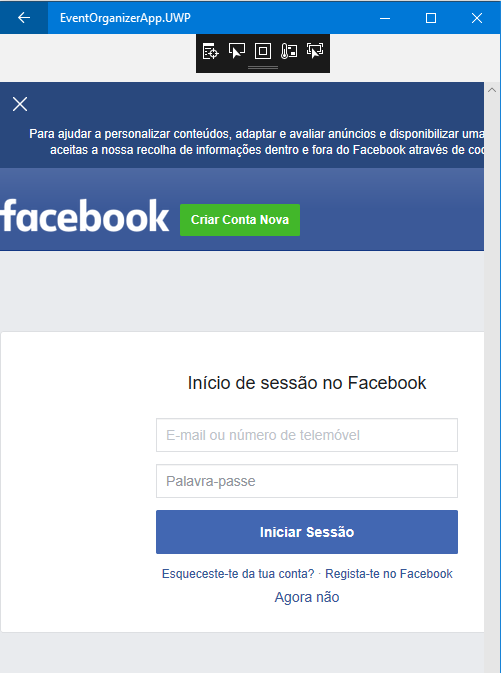
\includegraphics[width=0.60\textwidth,height=0.50\textheight]{./Chapter3/Figures/ClientAppScreenShots/Signup01}
	\caption{User Signup Screen}
	\label{fig:UserSignupScreenShot}
\end{figure}

\newpage
Users are redirected to the facebook login page to signup. It's possible to use \textit{Facebook} as an identity provider.
Once a user is signed in, it has the ability to create an event, giving its Title and Description, also the start and end dates. After the event is created, it can add its initial expenses/items so the invited users know if they need to pay for anything in advance, and how much.

Figure~\ref{fig:CreateEvent} illustrates the \textit{Event creation} operation.

\begin{figure}[!ht]
	\centering
	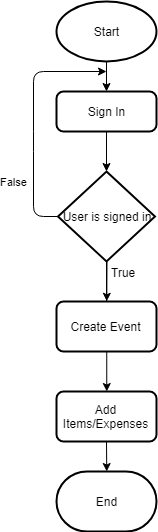
\includegraphics[width=0.25\textwidth,height=0.50\textheight]{./Chapter3/Figures/Flowcharts/CreateEventFlowChart}
	\caption{Create Event Flowchart}
	\label{fig:CreateEvent}
\end{figure}

\newpage

Figure~\ref{fig:CreateEventScreenShot} illustrates the \textit{Event creation} screen.

\begin{figure}[!ht]
	\centering
	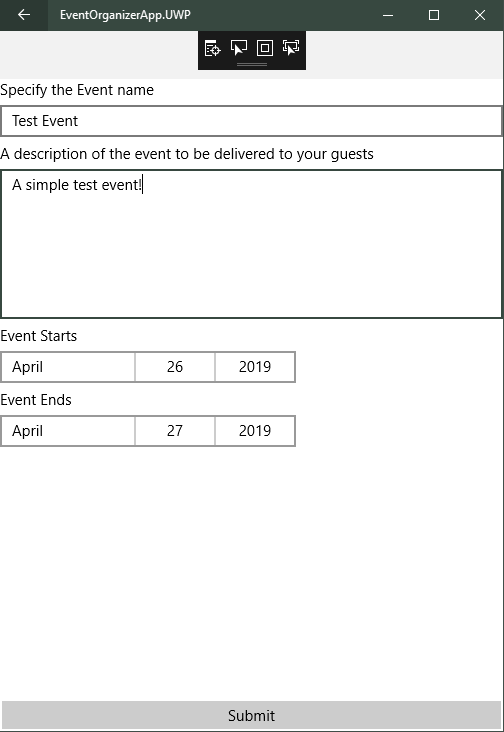
\includegraphics[width=0.60\textwidth,height=0.50\textheight]{./Chapter3/Figures/ClientAppScreenShots/CreateEvent04}
	\caption{Event Creation Screen}
	\label{fig:CreateEventScreenShot}
\end{figure}

\newpage

To add an item the user has to choose an event and then specify a title, description, price (if the item has a price) and it's type (types can be: \textit{Food}, \textit{Drink}, \textit{Decoration}, \textit{Taxes} and \textit{Others}).

Figure~\ref{fig:ItemCreationScreenShot} illustrates Item Creation.

\begin{figure}[!ht]
	\centering
	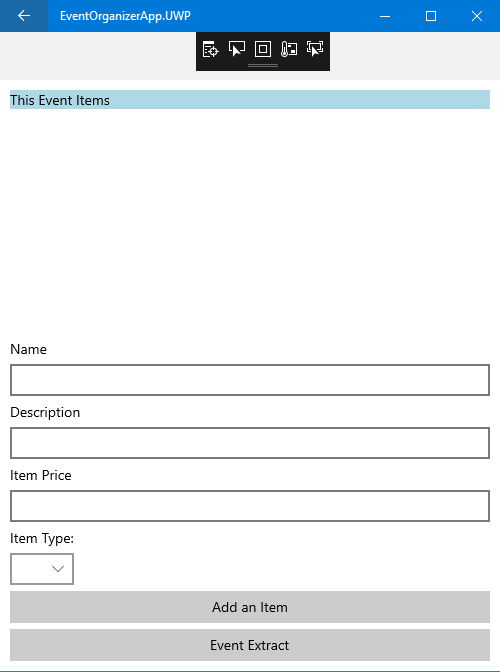
\includegraphics[width=0.60\textwidth,height=0.50\textheight]{./Chapter3/Figures/ClientAppScreenShots/AddItem_08}
	\caption{Item Creation Screen}
	\label{fig:ItemCreationScreenShot}
\end{figure}

\newpage

When items are created in the event a guest can see the event extract. This screen will present to the guest who is paying for what items and how much.

By selecting an item, inputting how much one has payed for it and clicking "Change Payed Value" an entry will be added to the event extract so other guests can see how much the others payed and how much it has to pay also.

Figure~\ref{fig:EventExtractScreenshot} illustrates Event Extract.

\begin{figure}[!ht]
	\centering
	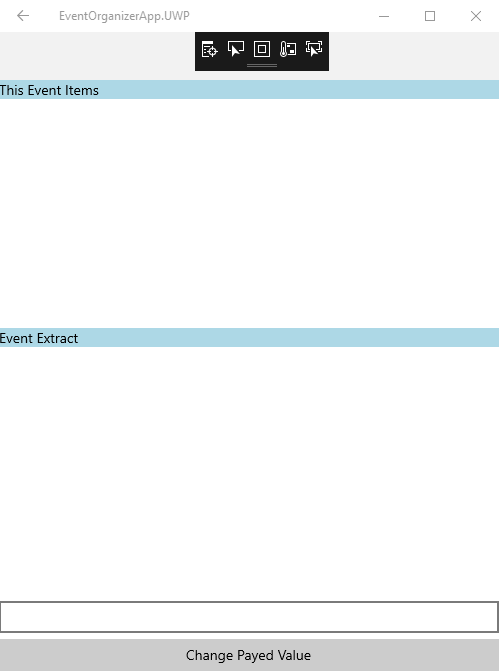
\includegraphics[width=0.60\textwidth,height=0.50\textheight]{./Chapter3/Figures/ClientAppScreenShots/Extract_01}
	\caption{Item Creation Screen}
	\label{fig:EventExtractScreenshot}
\end{figure}



\newpage

After the user has at least one event created it can see all the events that it created until now and when the user chooses an event, it can list and edit items aswell as invite users:

Figure~\ref{fig:EditEvent} illustrates the Event edit.

\begin{figure}[!ht]
	\centering
	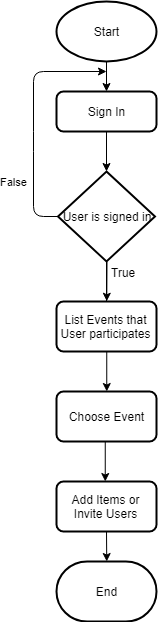
\includegraphics[width=0.25\textwidth,height=0.50\textheight]{./Chapter3/Figures/Flowcharts/EditEventFlowChart}
	\caption{Edit Event Flowchart}
	\label{fig:EditEvent}
\end{figure}

\newpage

Figure~\ref{fig:EditEventScreenShot} illustrates the Event edit.

\begin{figure}[!ht]
	\centering
	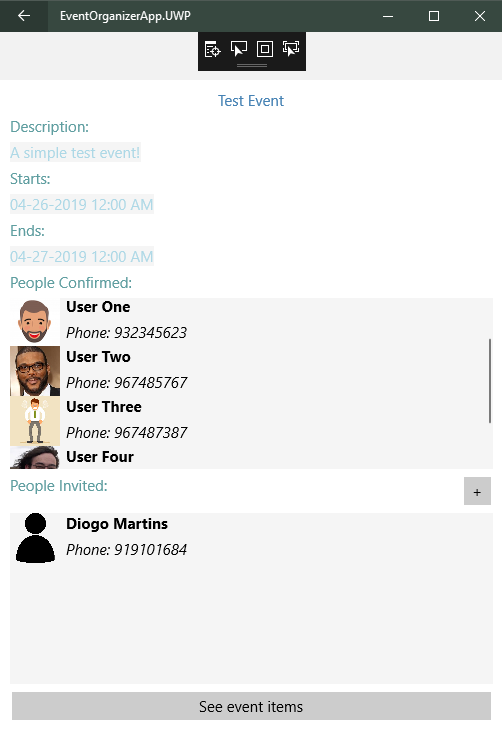
\includegraphics[width=0.60\textwidth,height=0.50\textheight]{./Chapter3/Figures/ClientAppScreenShots/Event13}
	\caption{Edit Event Screen}
	\label{fig:EditEventScreenShot}
\end{figure}

\newpage

It's also possible to add Tasks to users. Tasks are something that have to be completed until a certain expiration date. Tasks are comprised of a name, description and expiration date. They are also associated with a user so when a task is assigned to one they receive a notification.

Figure~\ref{fig:AddTaskToEvent} illustrates adding a Task to an Event.

\begin{figure}[!ht]
	\centering
	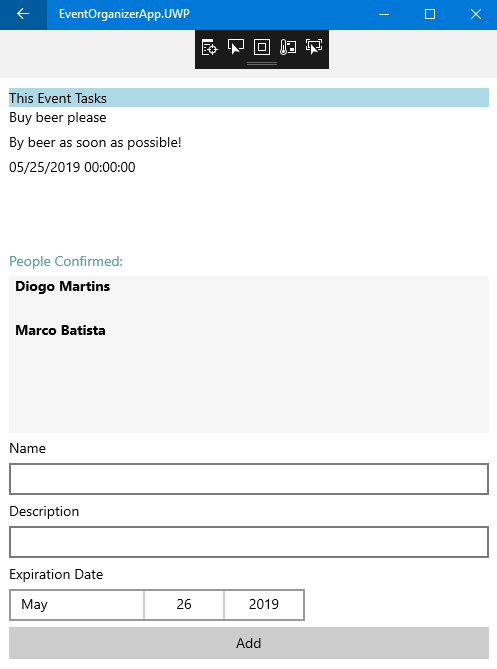
\includegraphics[width=0.60\textwidth,height=0.50\textheight]{./Chapter3/Figures/ClientAppScreenShots/AddTask_01}
	\caption{Edit Event Screen}
	\label{fig:AddTaskToEvent}
\end{figure}

\section{Events Web API}

The design of the API follows a REST approach over HTTP. This was decided so that the client/server side of the project can be \textit{scalable} and \textit{loosely coupled}, meaning that in the future, more clients for this API can be developed without the need to change anything to accommodate them.

%In order to try to decouple the server side from the client even more a \textit{Hypermedia As The Engine of Application State}, HATEOAS for short, component is also being considered as this would allow for the clients of the API to navigate it by using the \textit{hypermedia} links obtained in the various responses.%

In the current version, the Events API has the endpoints presented in Figure~\ref{fig:Endpoints}.


\begin{figure}[!ht]
	\centering
	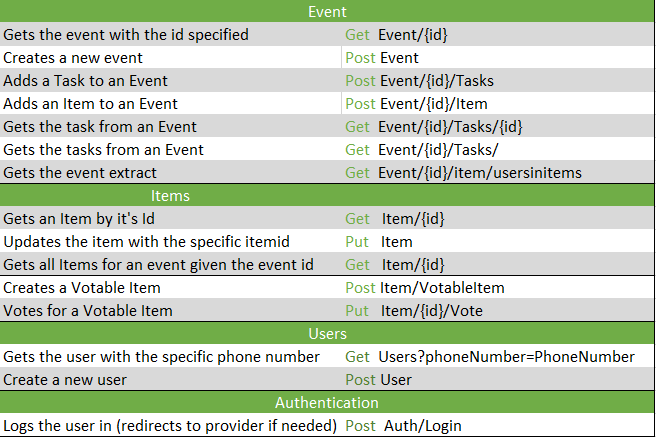
\includegraphics[width=1\textwidth,height=.45\textheight]{./Chapter3/Figures/EventsAPI_Endpoints}
	\caption{Events API endpoints in use by client application}
	\label{fig:Endpoints}
\end{figure}


The API is using Entity Framework, ADO.NET as the technologies to access data of the groups PostgreSQL database.

\newpage



\subsubsection{Implementation of the API}

\paragraph{Basic API structure}

The API, as mentioned earlier, is based on .NET Core. The controllers are called by the Http requests and the services that they use are initialized by the Dependency Injection engine that the framework provides. The dependencies are all configured on the Startup.cs file of the project.
The services contain all the business logic of the API and when they need to reach data to operate upon these call the methods exposed by the repository wrapper implemented in the API.

The repository wrapper allows for easy access to data repositories, being similar to a chest of items where one can get all of the data they need centralized in one class.

All of the repositories extend RepositoryBase<T> which exposes all the \gls{crud} operations while allowing for deferred execution when querying the database. Deferred execution allows for creating the query and only executing it against the database when a terminal method is called (for example .ToList()). This allows for a reduction of the queries ran on the database meaning it's possible to get all the data from a custom query only on one travel to the database server.


\paragraph{Logging}

The API allows for logging by using a group implemented Logging Provider and adding it to the Startup on configuration using \textit{ILoggerFactory}. The logging level is controlled by the appsettings file of the project where there are 7 levels:

\begin{itemize}
	\item Trace
	\item Debug
	\item Information
	\item Warning
	\item Error
	\item Critical
	\item None
\end{itemize}

Logging is called (or not) automatically by the platform according to the level defined in the settings.

In case of an occurrence of an unhandled exception there is an ErrorController than has an Error method that is a generic exception handler. This exception handler returns a 500 Http Status Code and before it returns to the user it sends an email to the groups application email box with a Message and StackTrace of the Exception. If the logging level is defined for every one except None it also gets logged to the logging database.

The logging database DAL is implemented using ADO.NET because of the fast execution of this technology while accessing a database. The tradeoff here is that this performance, which allows for the logging to be fast and less impact-full of the API performance overall, comes at a cost of the flexibility and code maintenance that Entity Framework provides.

\paragraph{Email Sending}

The email sending is used as the main notification system. It is used in the following situations:
\begin{itemize}
	\item When a user is registered an email is sent to its mailbox
	\item Upon the creation of an item or a task (sending the task to the person whom that task was assigned too)
	\item Sent to the group's mailbox when an Exception happens.
\end{itemize}

for when a new user is registered (sending a welcome email to the user mailbox) and on an unhandled exception.
The methods defined on this service are asynchronous methods so they run in the background as SMTP communication usually isn't very fast so this way the API overall performance is not impacted a lot in a negative way. The class the group is using to send emails is \textit{SmtpClient} and it's configuration is given by the appsettings file. The email provider the group is using is \textit{Outlook}.


\paragraph{ModelState Validation}

This API takes advantage of the technology of model validation present in the framework. This validation technology goes by the name of ModelState Validation. This technique consists on decorating the models used by the client application with Data Annotations.
These Data Annotations are placed in the properties of the model as Attributes. These can define if a property is required, what is the maximum length of a property (for example, in case of a string), the value range, etc…
The client application sends the model and when the request reaches the web API controller, one can check if the model sent by the client app is valid, by calling ModelState.IsValid, before sending the request to the other layers of the API (service, data, etc…).
If ModelState.IsValid returns true, then the model obeys to all validations described in the data annotations. However, if false, the request isn’t sent to the other layers, and on the response a body containing the validation errors will be sent (accompanied by a HTTP 400 – Bad Request – status code). These validation errors will help the client understand what is wrong with it’s request so they can correct it.

\section{Music Web Api}

The \textit{Music Web API} is a set of definitions that aim to unify music providers by having them expose common functionalities through a single \textit{Web API definition}.

\subsection{Structure}
The \textit{Music Web API} repository contains three main projects that are:

\begin{itemize}
	\item MusicWebApi – This project contains the interfaces that need to be implemented in order to follow the Music Web Api definition.
	
	\item MusicWebApi.Client – .NET Standard project that eases the use of Music Web Api Services by abstracting HTTP requests in simple method calls.
	
	\item MusicWebApi.Models – Another .NET Standard project shared by the first two containing the model objects for the API requests and responses.
\end{itemize}

In addition to these projects there are also projects that contain the implementations of the \textit{Music Web API}, such as \textit{SpotifyMusicWebApi}, an implementation for the popular Spotify music service.

\subsection{Definition}
As previously mentioned, the \textit{Music Web API} is an API definition for services that wish to expose the functionality of music providers, existing or native, in a uniform and standard interface.

Music applications can make use of this if there is a need to have multiple music providers without having to create multiple user interfaces or API access layer implementations. This can prove useful in both the maintainability of the code by keeping it uncluttered and centralized (only one API access service is needed) and in keeping the application easily expandable simply by adding to the music services available, without the need of big code changes.

The following diagram exemplifies the functionality of the \textit{Music Web API} ecosystem described earlier:

\begin{figure}[!ht]
	\centering
	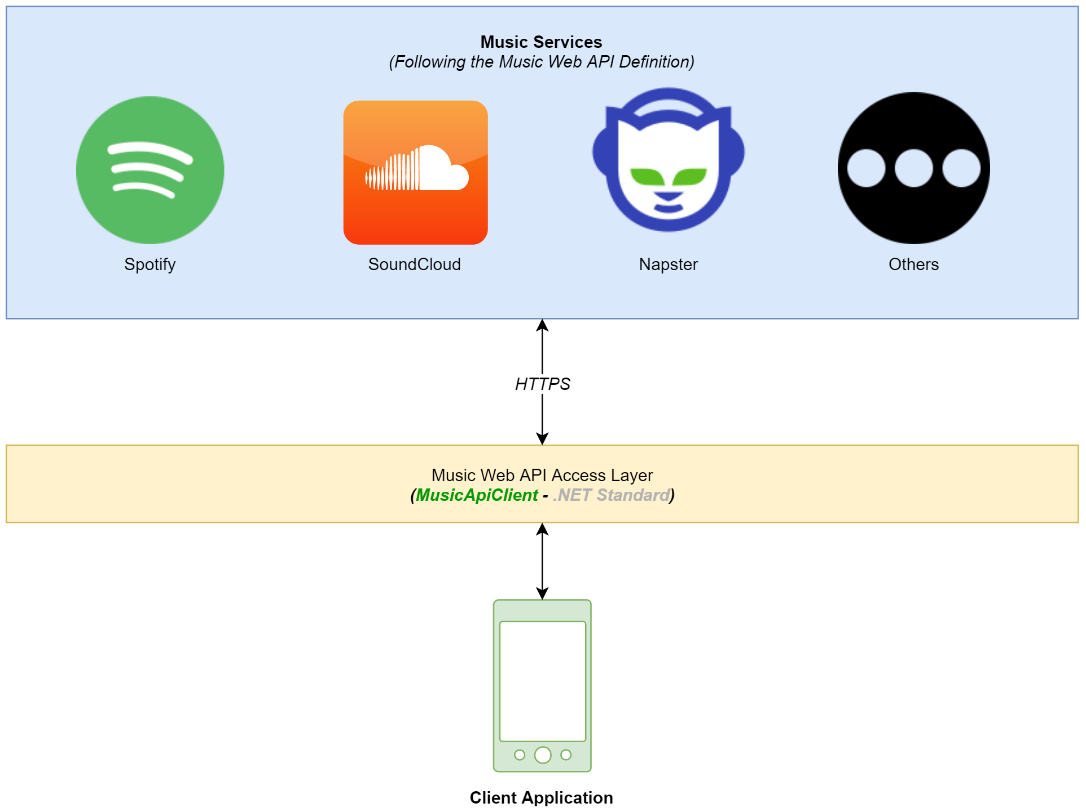
\includegraphics[width=1\textwidth,height=.45\textheight]{./Chapter3/Figures/MusicWebApi/MusicApiDiagram.png}
	\caption{Diagram of the Music Web API functionality}
	\label{fig:MusicApiDiagram}
\end{figure}

\begin{figure}[!ht]
	\centering
	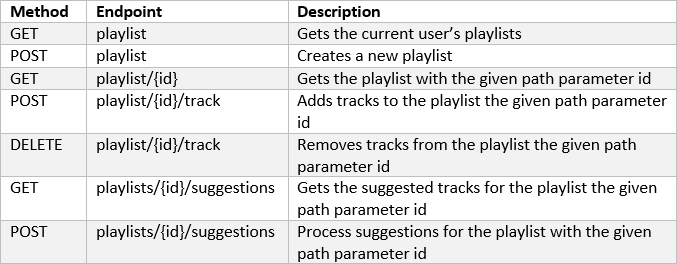
\includegraphics[width=1\textwidth,height=.20\textheight]{./Chapter3/Figures/MusicWebApi/PlaylistControllerTable.png}
	\caption{Playlist Controller}
	\label{fig:PlaylistControllerTable}
\end{figure}

\begin{figure}[!ht]
	\centering
	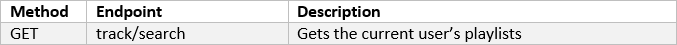
\includegraphics[width=1\textwidth,height=.025\textheight]{./Chapter3/Figures/MusicWebApi/TrackControllerTable.png}
	\caption{Track Controller}
	\label{fig:PlaylistControllerTable}
\end{figure}

The decision to keep the \textit{create playlist} and \textit{add tracks to playlist} endpoints working with the POST method instead of PUT was made because the \textit{Music Web API} definition cannot guarantee that, in the case where implementations use third party providers such as Spotify, the creation and addition of tracks is idempotent.

Although it makes the API less fault tolerant overall, it is a necessary trade off to make it broader by supporting implementations that use third party services.

\subsection{Authentication and authorization}
All music services that follow the definition \textit{Music Web API} must use the industry-standard protocol, OAuth 2.0, for authorization.

As such among the three controller interfaces in the MusicWebApi project an AuthController can be found. This controller has only two methods, one that begins the authentication flow for the user and another that serves as a redirect URI that must resolve the code and return a \textit{TokenResponse} object, which represents the standard OAuth 2.0 response, in the HTTP body.

\subsection{Client}
The client project allows for safer calls to a Music Web Api service by having methods that receive and return the exact model objects and build the appropriate HTTP requests. This makes applications that use these services cleaner and faster to develop, only needing to import the nugget package for this client and call the methods wanted.

\section{Client Application}

The initial plan for the client application was \textit{"a mobile application, using the \textit{Android} platform. The development environment will be .NET with the \textit{Xamarin} SDK."}. The group decided to use the Xamarin Forms variation of the environment since it has two advantages when compared to Xamarin Native:

\begin{itemize}
	\item The ability to share similar UI between two different platforms (in addition to application code);
	
	\item Easier maintenance since even more code is shared.
\end{itemize}

The group decided it was best to sacrifice application size (as this is the biggest con to Xamarin Forms) for better code organization and overall looks.

This decision also made it so there are now two client applications instead of just one. Right now it's possible to run the event organizer client application on both Android and UWP/Windows.

The platform supports the current operations:

\begin{itemize}
	\item Events - Create events;
	
	\item Items/Expenses - Addition of Expenses to an event;
	
	\item Tasks - Add tasks;
	
	\item Events - Cancel an event;
	
	\item Register Users - Registering users using authentication providers (\textit{Facebook})
	
	\item Invites - Invite users to participate in an event;
	
	\item Add Payment - Associate payment with a certain item and see the current extract of the event
\end{itemize}




\subsubsection{Implementation of the client app}

\paragraph{Layout and basic application structure}

This application as stated earlier is implemented using Xamarin Forms. This toolkit serves as our view engine for the application and suggests ways of organizing the client application so code can be reused between platforms.

The application has Content Pages that are the Views of the app. These are written using \textit{Extensible Application Markup Language} (XAML) which is a declarative markup language that allows to create the user interfaces for the application. These are written as files with the ".xaml" extension.
\newline
The XAML content pages have a .cs file associated with them that allow C\# code to be written to them by subscribing to events that are exposed by the Xamarin Forms platform.
This is simillar to ASP.NET's \textit{Web Forms}.

For example, when navigating between views there is a concept of "Push" and "Pop". Push meaning going forward and Pop going backwards in the page navigation.

When one is "Pushing" to a new view that view needs to be instantiated with the \textit{new} operator, executing the views ctor. The constructor shouldn't have code that takes time to complete in its body, only layout changes or event declaration should happen here, for example.

If one has to, for example, call the API when navigating to a new view one should subscribe to the \textit{OnAppearing} method which is called when the view is rendered on the target device.

\paragraph{Local Notifications}

Local notifications are handled with the help of a Xamarin Plugin called \textit{Xam.Plugins.Notifier}. This plugin allows for cross-platform local notification handling by exposing three methods to the programmer.
The group decided to use this plugin because of it's simplicity and the easiness of allowing the same notifications working for all platforms, in this case, UWP and Android. 
However there are some limitations with this plugin:



\begin{itemize}
	\item There is no way to get a list of the current notifications of the App;
	
	\item The latest (stable) version of the Nuget package present on the GitHub repo, as of 2019-05-18 is not working with scheduled notifications on UWP (meaning the group had to search the github repo of this plugin and on pull request \#43 https://github.com/edsnider/localnotificationsplugin/pull/43 this was fixed).
	
	
\end{itemize}

\newpage

The way the group handled the cancelling of scheduled notifications was to save the notifications according to an Id that could be easily retrieved when canceling, by giving the object that caused the notification to happen and an id:

These are the method signatures that handle this problem:
\begin{itemize}
	\item public void AddNotificationCountByObjectAndId<T>(T obj, int id, int count)
	where T : class - for adding notifications
	
	\item public void CancelNotificationByObjectAndId<T>(T obj, int id)
	where T : class - for cancelling notifications
	
	
\end{itemize}


For example if one wanted to add two notifications for an Event one would pass the EventModel object and its Id. This would save a configuration on the device after scheduling the notifications and if you wanted to cancel all of the notifications you would call CancelNotificationByObjectAndId with the same parameters that were supplied to an earlier call to AddNotificationCountByObjectAndId.

%Note that with this implementation it's not possible to cancel a specific notification with this implementation. 

Note that with this implementation it's not possible to cancel a specific notification. In case one wanted to cancel one it can be done by cancelling all notifications for a specific object and then creating new ones.

The handling of saving the configuration is done with the help of Xam.Plugins.Settings as used in other parts of this projects client application.

\paragraph{API Request Handling}

The application requests the groups API using a Request Service that is designed using \textit{HttpClient} and a class that the group implemented called NetworkService. This NetworkService class in conjunction with \textit{Polly} exposes a "Retry" method that allows for an arbitrary number of attempts of requesting the API in case a network communication fails, while allowing the group to execute a function on each attempt (for example, this can be used on a case where the user could be warned about the operation taking longer than usual). However the Request Service only uses the Network Service on GET methods because of the retry being a problem on non idempotent operations, which could cause inconsistencies to the application state.

\paragraph{Permission Handlers}

The maps and contact providers are implemented with permission handling in mind. Users might be prompted to grant permission to a functionality in the application, and the application should behave accordingly to the granting or denying of the permission.
On Android permission handling is different from other platforms, as on the user decision it calls a method on the MainActivity class of the application, meaning that the programmer will lose context from the page that requested the permission for a specific functionality.
To solve this the providers that require permissions have interfaces that expose callback setters, so immediately after the user grants or denies permission, there is behavior attached to its choice (for example, going back in the navigation stack when a user denies access to something).
Callback setters are useful and flexible because they separate the concerns to the provider. For example, after the user grants permissions to the contact list, it should be provided on the screen. For this functionality you set a callback to be executed after the granting of the permission by the user.
On UWP this isn’t needed, as the permission checking is not based on calling a method on another class. The UWP API normally exposes methods that return the permission status on the fly and then ask the user if the application does not have permission.
As a side note there is a Xamarin plugin for handling permissions called Plugin.Permissions. However, this plugin, by analyzing its source code, is somewhat heavy on the performance side, as to handle the permission architecture of android there is a need to use locking mechanisms to synchronize the permission request and its subsequent status.


\paragraph{Location/Maps}

The definition of the location of the event is supported by a plugin by the name of Xamarin.Forms.Maps. This plugin allows for the cross-platform integration of maps in a mobile application, providing a simple to use interface that is common to every platform.
The plugin is cross-platform, however, for each platform there is a different map provider:

\begin{itemize}
	\item Android – Google Maps map provider
	\item UWP – Bing map provider
	\item iOS – Apple maps map provider
\end{itemize}


However, when using a map provider, the application needs to ask the user for permission (mainly for location). This was handled by creating a wrapper around each provider and supplying instances to the cross-platform project of the application via dependency injection.
These wrappers handle permission handling as well as every map operation possible that the application needs to support (moving the map to a specific location, showing a dialog when the user doesn’t give permission for map usage, adding pins on the map, etc…).
The group implemented the map feature for the Android and UWP platforms.
As seen in the contacts provider, handling permissions on Android is particularly hard compared to other platforms. The Android runtime calls a specific method in the main activity to handle permissions, hence the need to pass page components to the maps provider (to call methods and implement functionality after the user grants permission.)

If the request for permission is denied, then the user is returned to the previous page. However, on the UWP application the settings page for permissions of the app is opened automatically, so the user can grant permission for map usage.

The search component of the map functionality of the application is provided by the OpenStreetMap API. The group decided to use this API as it is free, easy to use (there’s not even a need for requesting an API key). The only restrictions there are for this API is that you shouldn’t abuse requesting it and it is obligatory to identify your application by providing a custom user-agent in the HTTP headers. The user searches an address, the results are presented, and after the user chooses one from the list, the coordinates are passed into the map provider (giving the opportunity for the user to save the event location).

\paragraph{Contacts}
When one is inviting a user to an event a list of contacts present in the invitee's device is shown. The list of contacts is brought with the help of contact providers and a Xamarin plugin called Xamarin.Forms.Contacts.
The Xamarin plugin is straightforward to use. This plugin provides a service and there is only need to call a method on that service. However this plugin does not handle permissions and it does not work on UWP. So the group implemented a "hybrid" solution with contact providers.
Contact providers offer an interface to implement contact functionality on multiple platforms.
This contact provider allows one to supply the list view that is going to hold the contacts to an instance of itself. This is especially useful for handling Android permissions.


\newpage
\subsection{Database}

The application and logging databases are being supported by PostgreSQL. The group choose this engine over others because this one is free and open-source, it also supports a wide range of operating systems and is usually faster to install and setup.

%This is the current data model:

Figure~\ref{fig:EAModel} illustrates the data model.

\begin{figure}[!ht]
	\centering
	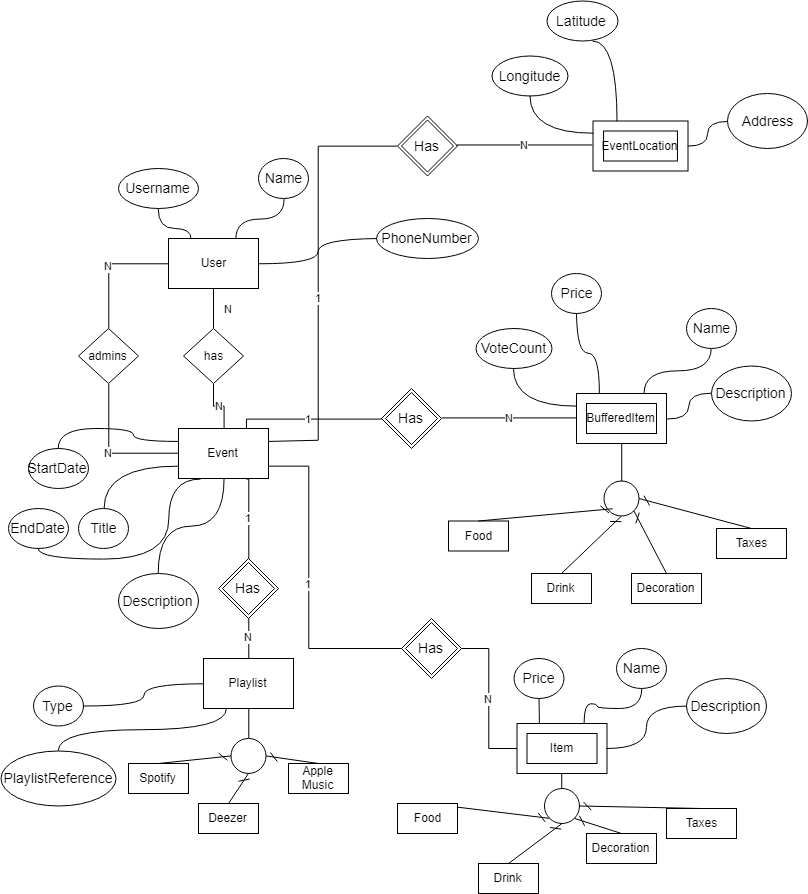
\includegraphics[width=0.75\textwidth]{./Chapter3/Figures/EventDatabase.png}
	\caption{Data Model}
	\label{fig:EAModel}
\end{figure}


\begin{itemize}
	\item Event - Represents the Events, has a Title, Description and Start/End dates of the event;
	
	\item Item - Represents the Items (or expenses) of the Event. Has a Name, Description, Price, State and it can have various types;
	
	\item Task - Represents the Tasks of the Event assigned to participants. Has a Name, Description, Expiration Date, State and references an event and a participant;
	
	\item BufferedItem - It is the same as the Items except it represents only the items that have been successfully approved by all members of the event (note the VoteCount field, it is incremented by 1 every time a user votes). When the VoteCount field value is the same as the number of users in an Event, the BufferedItem gets moved to the Item table;
	
	\item Playlist - Represents a Playlist, has a reference (URL to the playlist itself) and a type (this type describes the service that provides the playlist. Example: \textit{Spotify});
	
	\item User - Describes a User, has a Name, Username and a Phone Number;
	
	\item EventLocation - Represent the Event location. Has an address, longitude and latitude.
	
\end{itemize}


The logging database is apart of the applicational one. This is because not only might the applicational database be in a different location from the logging one but the logs can grow exponentionally, affecting storage and performance of the applicational one if the log table was in the same database.

The logging database only hosts one table on the default schema. The table is called EventLog and it represents logs. It is comprised of an EventId (type of log), LogLevel, Date, Message and StackTrace (these last two are only present in case of an exception logging):

Figure~\ref{fig:LoggingModel} illustrates the logging database model.

\begin{figure}[!ht]
	\centering
	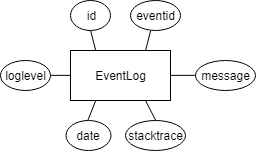
\includegraphics[width=0.75\textwidth]{./Chapter3/Figures/Logging_Db.png}
	\caption{Data Model}
	\label{fig:LoggingModel}
\end{figure}

%\textbf{NOTE: All of these tables have a unique id that is an autoincremented/serial upon insertion integer.}

\textbf{Note:} All of these tables have a unique id that is an autoincremented/serial upon insertion integer.


